\documentclass[12pt]{article}
\usepackage[utf8]{inputenc}
\usepackage{amsmath, amssymb, amsfonts}
\usepackage{geometry}
\usepackage{booktabs}
\usepackage{enumitem}
\usepackage{caption}
\usepackage{tikz}
\usepackage{pgfplots}
\pgfplotsset{compat=1.15}
\geometry{margin=1in}
\setlist[enumerate]{leftmargin=*}

\title{Solutions -- Practice Problem Set 1\\ \vspace{15pt} \large ECON 101 -- Macroeconomics}
\author{}
\date{Winter 2026}

\begin{document}
\maketitle


\begin{enumerate}
\item \textbf{Scarcity and Trade-offs} \\
Scarcity means resources (time, income, natural resources) are limited relative to wants. Because of scarcity, choosing one option requires forgoing another (\emph{trade-off}), and the \emph{opportunity cost} of any choice is the value of the best alternative given up. \\
\textbf{Examples.}
\begin{itemize}
  \item \emph{Student time:} Spending three hours studying economics means forgoing three hours working for pay or relaxing. The opportunity cost of studying is the wage (or leisure) foregone.
  \item \emph{Budget trade-off:} Buying a \$1{,}200 laptop today may force postponing a vacation. The opportunity cost of the laptop is the next-best use of that \$1{,}200 (e.g., part of tuition or the vacation).
\end{itemize}
\textbf{Why fundamental?} Every decision requires comparing marginal benefits with marginal opportunity costs, precisely because resources are scarce.

\item \textbf{Economic Models} \\
\textbf{Why use models?} Models simplify reality to isolate causal mechanisms (e.g., how price affects quantity demanded). Assumptions (ceteris paribus) help derive clear, testable predictions. They guide measurement and counterfactual analysis (``what if'' policy experiments). \\
\textbf{Strengths.} Clarity, internal consistency, predictive discipline, and portability across contexts. \\
\textbf{Limitations.} Omitted variables/institutions, parameter instability (behavior may change with policy), measurement error, and potential mismatch between assumptions and context. Good practice: use models as \emph{maps}, validated and refined with data.

\item \textbf{Positive vs. Normative Analysis} \\
\textbf{Positive (descriptive/testable):} ``A \$10 billion increase in government spending raises real GDP in the short run.'' This can be confronted with data. \\
\textbf{Normative (prescriptive/value-laden):} ``The government \emph{should} increase spending to reduce unemployment.'' This depends on goals (equity vs. efficiency) and value judgments. \\
\textbf{Why distinction matters.} It separates evidence-based claims from value-based recommendations, clarifying where economists agree (facts/estimates) and where disagreement stems from different social objectives.

\item \textbf{Specialization and Trade (Comparative Advantage)} \\
\textbf{Key logic:} Even if one party is absolutely more productive in all goods, each can gain by specializing in the good with the \emph{lower opportunity cost} and trading for the other good. \\
\textbf{Steps:} (i) Compute opportunity costs in each country/person. (ii) Assign production to the activity with lower opportunity cost. (iii) Choose a mutually beneficial terms of trade between the two opportunity costs. (iv) Both consume beyond their individual PPFs. \\
\textbf{Intuition:} Specialization aligns production with relative efficiencies, expanding total output; trade reallocates that surplus to improve both parties' consumption possibilities.

\item \textbf{PPF: Points Inside/On/Outside} \\
\textbf{Inside the PPF:} Feasible but inefficient (unused labor/capital or misallocation). \emph{Example:} Producing 300 bushels of wheat and 60 cars when available resources could produce 400 bushels of wheat and 70 cars. \\
\textbf{On the PPF:} Feasible and productively efficient (cannot produce more of one good without less of the other). \emph{Example:} A point consistent with full employment and best-known technology. \\
\textbf{Outside the PPF:} Currently unattainable with given resources/technology. \emph{Example:} 900 bushels of wheat and 120 cars when the economy's maximum combinations fall short; attainable only with growth, trade, or technology improvements.

\end{enumerate}


\begin{enumerate}[resume]
\item \textbf{Opportunity Cost Calculation} \\
\textbf{Given:} Essay takes 5 hours and yields benefit valued at \$80. Working pays \$15/hour. \\
\textbf{(a) Opportunity cost of writing the essay.}
\[
\text{Wage foregone} = 5 \text{ hours} \times \$15/\text{hour} = \$75.
\]
So the opportunity cost of writing the essay is \$75 (best alternative given up). \\
\textbf{(b)}Compare benefit (\$80) to opportunity cost (\$75). Net gain from essay:
\[
\$80 - \$75 = \$5 > 0.
\]
She should write the essay if she values the grade improvement at \$80 (and there are no other relevant costs/benefits). A sensitivity note: if her true valuation were \(<\$75\), working would dominate.


\newpage

\item \textbf{PPF and Trade-offs} \\

\[
\begin{array}{c|cc}
\text{Comb.} & \text{Wheat} & \text{Cars}\\\hline
A & 0 & 100\\
B & 200 & 90\\
C & 400 & 70\\
D & 600 & 40\\
E & 800 & 0
\end{array}
\]
\textbf{(a)} The plot below places Wheat on the horizontal axis and Cars on the vertical axis. The five observed efficient points are connected with a smooth, concave envelope, reflecting increasing opportunity cost.

\begin{figure}[h!]
\centering
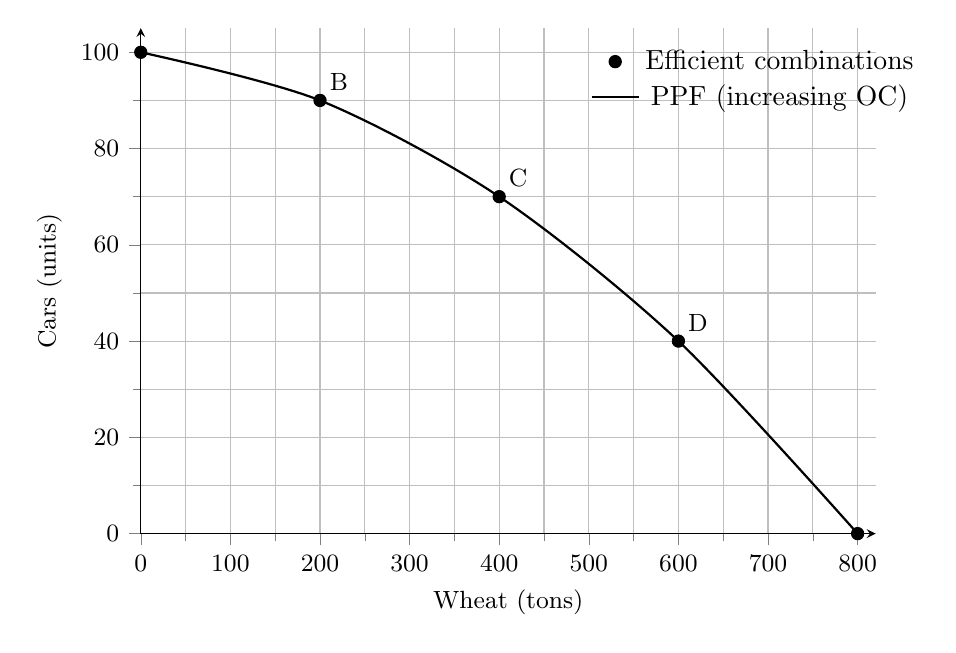
\begin{tikzpicture}
\begin{axis}[
  width=0.9\textwidth,height=8cm,
  xlabel={Wheat (tons)},ylabel={Cars (units)},
  xmin=0,xmax=820,ymin=0,ymax=105,
  axis lines=left, grid=both, minor tick num=1,
  tick align=outside,
  legend style={draw=none, fill=none, at={(0.6,0.98)}, anchor=north west},
  label style={font=\small},
  ticklabel style={font=\small}
]
\addplot[only marks, mark=*, mark size=2.2pt] coordinates {(0,100) (200,90) (400,70) (600,40) (800,0)};
\addlegendentry{Efficient combinations}
\addplot[thick, smooth] coordinates {(0,100) (200,90) (400,70) (600,40) (800,0)};
\addlegendentry{PPF (increasing OC)}
\node at (axis cs:0,100) [anchor=east] {\small A};
\node at (axis cs:200,90) [anchor=south west] {\small B};
\node at (axis cs:400,70) [anchor=south west] {\small C};
\node at (axis cs:600,40) [anchor=south west] {\small D};
\node at (axis cs:800,0) [anchor=north] {\small E};
\end{axis}
\end{tikzpicture}
\caption*{\small Figure 1. Production Possibilities Frontier for Wheat and Cars.}
\end{figure}

\textbf{(b) Opportunity cost from B to C.} Moving \(B\to C\): Wheat increases by \(+200\), Cars decrease by \(-20\).
\[
\text{OC of } +200 \text{ wheat} = 20 \text{ cars}\quad \Rightarrow \quad 0.10 \text{ car per ton of wheat.}
\]
Equivalently, \(1\) car costs \(10\) tons of wheat at this margin. \\
\textbf{(c) Is OC increasing?} Along each segment:
\[
\begin{aligned}
A\to B:&\ 0.05 \ \text{car/ton}\quad
B\to C:&\ 0.10 \ \text{car/ton}\quad
C\to D:&\ 0.15 \ \text{car/ton}\quad
D\to E:&\ 0.20 \ \text{car/ton}
\end{aligned}
\]
Opportunity cost rises monotonically as wheat output expands: \textbf{increasing} OC.


\newpage
\item \textbf{Comparative Advantage and Trade} \\

\[
\begin{array}{c|cc}
 & \text{Cloth} & \text{Wine}\\\hline
\text{Alpha} & 60 & 30\\
\text{Beta} & 40 & 20
\end{array}
\]
Assume linear PPFs (constant OC). \\
\textbf{(a) Opportunity costs.} \\
Alpha: \(1\) cloth \(=0.5\) wine; \(1\) wine \(=2\) cloth.\\
Beta: \(1\) cloth \(=0.5\) wine; \(1\) wine \(=2\) cloth. \\
\textbf{(b) Comparative advantage.} Identical OCs $\Rightarrow$ \textbf{neither} country has a comparative advantage. \\
\textbf{(c) Gains from trade?} With identical OCs and CRS, \emph{no specialization gains} arise at terms of trade equal to the common OC. 


\end{enumerate}

\end{document}
